\chapter[Solução Geral]{Solução Geral}
\section{Escopo}
% Descrever projeto e especificar protótipos caso exista
O projeto PillWatcher consiste na construção de um dispensador automático de medicamentos sólidos, o qual terá a função de armazenar e realizar a separação da dose medicamentosa individual nos horários pré-estabelecidos pelo médico. Além do mais, o projeto possuirá uma aplicação \textit{mobile} e um conjunto de microsserviços únicos como o servidor de gerenciamento da interface com o usuário e o gerenciamento da coleta de dados.

Existirá a comunicação entre o dispositivo e o aplicativo, uma vez que, este será elaborado para realizar o cadastro de enfermeiros, pacientes e medicamentos, além de enviar avisos quando se aproxima do horário da medicação. O aplicativo informará a quantidade de todos os medicamentos, avisando a reposição quando necessária.

O compartimento superior do dispositivo contará com uma entrada para realizar o abastecimento de medicamentos no estoque de contêineres. Enquanto que, no compartimento frontal, existirá uma saída para a retirada dos recipientes com a medicação correta para cada paciente. Entretanto, é necessária uma autenticação do corpo técnico de médicos, enfermeiros e cuidadores das clínicas geriátricas para permitir o acesso a esses compartimentos.

Visando uma melhor compreensão do projeto, foram elaboradas soluções particulares de cada área do projeto afim de garantir a elaboração correta do produto final.

\section{Lista É/ Não É}
A Lista É/ Não É que define o projeto PillWatcher encontra-se no Apêndice \ref{Lista_app}
\section{Solução Estrutural}
% Cada frente deve adc os subtópicos que acharem pertinentes
A abordagem estrutural compreende um sistema composto por um conjunto de estruturas críticas:

\begin{enumerate}
\item \textbf{Estrutura principal:}
responsável pela proteção dos demais subsistemas de esforços físicos e condições adversas de temperatura, pressão e umidade além de impedir que o usuário entre em contato com os medicamentos sem autorização. A carcaça será constituída de:
\begin{enumerate}
    \item Conjunto de tubos perfil quadrado, em formato de gaiola estrutural, proporcionando resistência estática e sustentação global das estruturas e de seus sistemas, assim como pontos de ancoragem e referência no projeto. As dimensões dos tubos são:
    \begin{itemize}
        \item Largura: 51mm;
        \item Comprimento: 51mm;
        \item Espessura de parede: 4,7mm;
        \item Material: Aço carbono SAE 1020;
    \end{itemize}
    
    \item Mancais de suporte dos fusos: Os mancais serão utilizados para ancorar os rolamentos dos fusos, produto que oferece suporte estrutural para os fusos e também conformidade com o movimento rotacional proposto pelos mesmos. Suas dimensões são:
    \begin{itemize}
        \item Comprimento: 30mm;
        \item Altura: 48mm;
        \item Diâmetro da circunferência externa: 48mm;
        \item Diâmetro do furo para o rolamento: 26mm;
        \item Espessura: 5mm;
        \item Material: Aço carbono SAE 1020;
        \item Diâmetro interno do rolamento: 16mm;
        \item Tipo de rolamento: Ponta de agulha;
    \end{itemize}
    
    \item Estrutura para suporte do atuador linear do recipiente dos copos, ancorada sobre a estrutura tubular próxima à esteira, com as seguintes especificações:
    \begin{itemize} 
        \item Largura: 103mm;
        \item Comprimento: 200mm;
        \item Espessura: 1,5mm;
        \item Material: Aço carbono SAE 1020;
    \end{itemize}
    
    \item Estrutura de suporte da esteira composto por engrenagens e eixos ancorados na estrutura tubular. Suas dimensões são:
    \begin{itemize}
        \item Diâmetro da engrenagem(sem dente): 18mm;
        \item Comprimento da engrenagem: 30mm;
        \item Altura do dente da engrenagem: 5mm;
        \item Diâmetro do eixo da engrenagem: 2,3mm;
        \item Comprimento do eixo da engrenagem: 89mm;
        \item Material: Plástico Polipropileno.
    \end{itemize}
    
    \item Estrutura de suporte para os motores de passo dos fusos, com as dimensões:
    \begin{itemize}
        \item Largura: 103mm;
        \item Comprimento: 60mm;
        \item Espessura: 1,5mm;
        \item Material: Aço carbono SAE 1020;
    \end{itemize}
    
    \item Estrutura de suporte para o motor DC da esteira, ancorada na estrutura tubular. As dimensões desse suporte são:
    \begin{itemize}
        \item Largura: 40mm;
        \item Comprimento: 50mm;
        \item Espessura: 1,5mm;
        \item Material: Aço carbono SAE 1020;
    \end{itemize}
    
\end{enumerate}


\item \textbf{Contêiner de medicamentos:} Estrutura responsável pelo abrigo e preservação dos remédios inseridos na máquina, divida em:
\begin{enumerate}
    \item Rampa seletora: Estrutura em formato circular com centro coincidente com o do contêiner, com um domo em formato de calota esférica no topo para que os remédios sejam direcionados às extremidades do contêiner. A rampa tem formato de cunha e é solidária ao domo. Com o movimento rotativo transmitido da engrenagem por meio de um eixo cilíndrico de extremidade hexagonal que se liga à porção inferior do domo, a estrutura de cunha com função de rampa rotaciona e empurra o comprimido para a zona intermediária.
    Especificações:
    \begin{itemize}
        \item Diâmetro do domo: 62 mm
        \item Raio de circunferência do topo do domo: 53 mm
        \item Altura do Domo: 16 mm
        \item Altura da rampa: 6 mm
        \item Angulação da rampa: 60º
        \item Comprimento circular da rampa: 177 mm
        \item Diâmetro do Domo com a rampa: 80 mm
        \item Material: Polipropileno
    \end{itemize}
    \item \textbf{Plataforma de seleção:} Peça cilíndrica posicionada abaixo da rampa seletora e fixada ao compartimento inferior por meio de parafusos. Na sua extremidade está localizado o furo retangular responsável pela seleção dos remédios do contêiner para transporte, as extremidades do furo são chanfradas e atuam como facilitadores para a descida dos remédios. No seu centro há um furo com um rolamento inserido e pelo qual passa a porção cilíndrica do eixo que movimenta a rampa seletora. A plataforma de seleção não apresenta movimento rotativo. As dimensões dessa estrutura são:
    \begin{itemize}
        \item Diâmetro da plataforma: 80 mm
        \item Altura da plataforma: 8 mm
        \item Área da seleção do medicamento: 164 mm$^2$
        \item Diâmetro do furo para o rolamento: 30 mm
        \item Diâmetro dos furos para fixação no compartimento inferior: 4 mm (3x)
        \item Tipo de rolamento: Rolamento usinado de agulhas com pista interna
        \item Material: Polipropileno
    \end{itemize}
    \item \textbf{Engrenagem com eixo:} Engrenagem helicoidal fabricada em peça única com um eixo escalonado em uma porção cilíndrica e uma extremidade com formato de prisma hexagonal que se encaixa à porção inferior do domo da rampa seletora. Na sua parte inferior, há um furo para o seu suporte.
    A porção cilíndrica tem diâmetro maior que a porção hexagonal, desta maneira, ela é inserida pelo fundo da montagem, através da base do compartimento inferior e da plataforma de seleção (cujo rolamento permite que a plataforma permaneça estática enquanto a rampa seletora se movimenta) e encaixada à rampa seletora. O movimento radial da engrenagem provém de um fuso, cujo eixo é perpendicular ao eixo da engrenagem, instalado solidário a um motor de passo.
    \begin{itemize}
        \item Módulo da Engrenagem: 4mm
        \item Número de dentes: 12
        \item Ângulo de pressão: 20º
        \item Diâmetro do furo da engrenagem: 10 mm
        \item Diâmetro da seção circular do eixo: 20 mm
        \item Comprimento da seção circular: 20 mm
        \item Lado da extremidade hexagonal: 8,66 mm
        \item Comprimento da extremidade hexagonal: 10 mm
        \item Material: Polipropileno
    \end{itemize}
    \item \textbf{Compartimento inferior:} Compartimento que funciona de base para a montagem do contêiner. Nele é fixada a plataforma de seleção e a parede cilíndrica do contêiner. Sua porção inferior possui dois furos, um central pelo qual o eixo da engrenagem passa e um na extremidade radial para a seleção do medicamento armazenado. Ele apresenta um pequeno macho de rosca na sua lateral para que ele se encaixe com um pequeno giro à base que sustenta cada fileira de contêineres, de forma semelhante ao que ocorre com o copo de um liquidificador.
    \begin{itemize}
       \item Diâmetro externo: 86 mm
        \item Espessura: 3 mm
        \item Altura: 50 mm
        \item Diâmetro do furo para passagem do eixo: 20 mm
        \item Diâmetro dos furos de fixação da plataforma de seleção: 4 mm (3x)
         \item Material: Polipropileno
\end{itemize}
    \item \textbf{Suporte da Engrenagem:} Pequena chapa retangular com extremidades arredondadas. Em seu centro há um pino que recebe uma arruela e se encaixa à porção inferior da engrenagem. Em cada uma das extremidades projeta-se um tubo pelos quais são passados os parafusos de fixação do suporte, estes se prendem à mesa de apoio utilizando uma porca.
    \begin{itemize}
        \item Comprimento do suporte: 128 mm
        \item Espessura do suporte: 6 mm
        \item Diâmetro do pino de suporte: 10 mm
        \item Comprimento do pino de suporte: 10 mm
        \item Diâmetro externo da arruela: 16 mm
        \item Espessura da arruela: 2 mm
        \item Diâmetro interno dos tubos de fixação: 6 mm
        \item Espessura dos tubos de fixação: 2 mm
        \item Altura dos tubos de fixação: 23 mm
         \item Material: Polipropileno
    \end{itemize}
    \item \textbf{Parede cilíndrica:} Chapa de pequena espessura feita de aço inoxidável curvada e soldada ou conformada mecanicamente até formar um cilindro. Encaixa-se no compartimento inferior em uma porção vazada da sua região superior. Em cima dela é encaixada uma tampa para garantir o melhor isolamento possível do contêiner.
    \begin{itemize}
        \item Diâmetro externo da parede cilíndrica: 83,4 mm
        \item Espessura da parede cilíndrica: 0,7 mm
        \item Altura da parede cilíndrica: 100 mm
         \item Material da parede cilíndrica: Aço inoxidável
         \item Material da tampa: Polipropileno
    \end{itemize}
    \item \textbf{Comporta do solenoide:} Pequena chapa de material polimérico e formato semelhante a um trapézio com as bases arredondadas e uma estrutura triangular de suporte. Posiciona-se na extremidade inferior do contêiner, abaixo do compartimento inferior e encontra-se normalmente fechada. Está fixada por parafuso a um solenoide com retorno por mola e recua quando necessária a liberação de um medicamento. O solenoide é aparafusado à mesa de apoio.
    \begin{itemize}
        \item Largura maior da comporta: 7 mm
        \item Largura menor da comporta: 6 mm
        \item Comprimento da comporta até o suporte: 16 mm
        \item Altura do suporte da comporta: 15,5 mm
        \item Espessura da comporta e do suporte: 3 mm
        \item Largura da fixação do suporte da comporta: 8 mm
        \item Diâmetro do furo da fixação do suporte da comporta: 3 mm
        \item Material: Polipropileno
    \end{itemize}
    \item \textbf{Base para fixação do contêiner:} Unida mecanicamente por quatro parafusos à mesa de apoio, possui um furo com rosca fêmea para o encaixe do compartimento inferior do contêiner, impedindo tanto seu movimento axial quanto radial.
    \begin{itemize}
        \item Diâmetro externo da base de fixação: 96 mm
        \item Espessura da base de fixação: 5 mm
        \item Diâmetro total com as abas para os parafusos: 124 mm
        \item Diâmetro dos parafusos de fixação: 6 mm
        \item Espessura das abas de fixação: 10 mm
        \item Material: Polipropileno
    \end{itemize}
\end{enumerate}
\item \textbf{Mesa de apoio:} Local responsável por estabelecer a sustentação do suporte e promover local de encaixe para os 25 contêineres. As dimensões dessa estrutura são:
\begin{itemize}
    \item Comprimento da mesa: 745mm;
    \item Largura da mesa: 200mm;
    \item Espessura: 3mm;
    \item Material: Aço carbono AISI 1020;
\end{itemize}
\item \textbf{Zona de transição:} Região onde haverá o cone de direcionamento para a medicação selecionada, com 25 canais de entrada e 1 canal de saída. Essa região compreende a união de 25 canais individuais com uma região de afunilamento, direcionando para a posição de despejo dos medicamentos. As dimensões dessa estrutura são:
\begin{itemize}
    \item Altura total do funil: 15cm;
    \item Diâmetro interno dos canais de entrada: 16mm;
    \item Espessura da parede dos canais de entrada: 2mm;
    \item Diâmetro do canal de saída: 15mm;
    \item Diâmetro do canal superior do funil: 17,7cm;
    \item Espessura da parede do funil: 1,5mm;
    \item Material do Funil: Nylon;
    \item Material dos canais de entrada: Mangueiras de silicone;
\end{itemize}
\item \textbf{Esteira:} Objeto utilizado para fazer o transporte do recipiente com os medicamentos selecionados para o compartimento frontal ou traseiro. Essa estrutura é formada por pequenas plataformas ligadas por pinos de aço inox, com dimensões especificadas abaixo:
\begin{itemize}
    \item Comprimento da plataforma: 82,5mm;
    \item Altura da plataforma: 19,9mm;
    \item Distância fura a furo: 38,1mm;
    \item Diâmetro dos furos: 6,35mm;
    \item Diâmetro dos pinos: 6,35mm;
    \item Material dos pinos: Acetal;
    \item Material da plataforma: Aço Inox AISI 304;
    \item Peso da plataforma e pino: 1 kg/m;
    \item Comprimento total da esteira: 1434mm;
\end{itemize}

\item \textbf{Reservatório de copos:} Local responsável por armazenar os recipientes dos medicamentos selecionados antes do uso. Essa estrutura está localizada em um plano adjacente a esteira, e há um auxilio por cantoneiras circulares, para que não haja movimento dos copos dentro da estrutura. As dimensões dessa estrutura são:
\begin{itemize}
    \item Altura total: 300mm;
    \item Largura: 60mm;
    \item Comprimento: 60mm;
    \item Espessura: 1,5mm;
    \item Diâmetro da cantoneira: 60mm;
    \item Altura da abertura dos copos: 35mm;
    \item Comprimento da abertura dos copos: 57mm;
    \item Material: Aço carbono SAE 1020;
\end{itemize}
\item \textbf{Copo dos medicamentos:} Recipiente responsável por resguardar os medicamentos selecionados pela Central de comando, que passaram pela Zona de Transição e são depositados sobre o mesmo, na posição inicial de despejo. Suas dimensões são:
\begin{itemize}
    \item Altura total: 30mm;
    \item Diâmetro externo: 50mm;
    \item Diâmetro do ressalto inferior: 55mm;
    \item Espessura da parede: 1,5mm;
    \item Altura do ressalto inferior: 1,5mm; 
    \item Diâmetro no ressalto interno superior: 44mm;
    \item Material: Polipropileno;
\end{itemize}

\item \textbf{Fuso de acoplamento:} Estrutura em formato helicoidal com passo de 10mm com coincidência central no eixo dos motores de passo de cada subgrupo, e fixado por meio de um rolamento dentro de um mancal de suporte, oposto ao motor de passo. As dimensões do fuso são:
\begin{itemize}
    \item Comprimento total: 765mm;
    \item Diâmetro do fuso: 16mm;
    \item Tipo do dente: Helicoidal;
    \item Passo do fuso: 10mm;
    \item Material: Plástico Polipropileno;
\end{itemize}
\item \textbf{Compartimento traseiro:} Área onde será efetuada a retirada dos recipientes com medicação extra (com falhas) pelo usuário. As dimensões desse compartimento são:
\begin{itemize}
    \item Altura: 80mm;
    \item Comprimento: 100mm;
    \item Espessura: 1,5mm;
    \item Diâmetro do eixo de abertura:
    \item Material: Aço carbono SAE 1020;
\end{itemize}
\item \textbf{Compartimento frontal:} Área onde será efetuada a retirada dos recipientes com medicação correta pelo usuário. As dimensões desse compartimento são iguais ao do compartimento anterior.
\end{enumerate}



\subsection{Formato da estrutura e CAD Preliminar}
Os desenhos estarão disponíveis no apêndice \ref{cad_preliminar}.

\subsection{Dinâmica de operação}

Após identificados os componentes do sistema, temos a exemplificação de seu funcionamento, feita preliminarmente via o fluxograma da figura \ref{fig:FEst}.

\begin{figure}[ht]
        \centering
        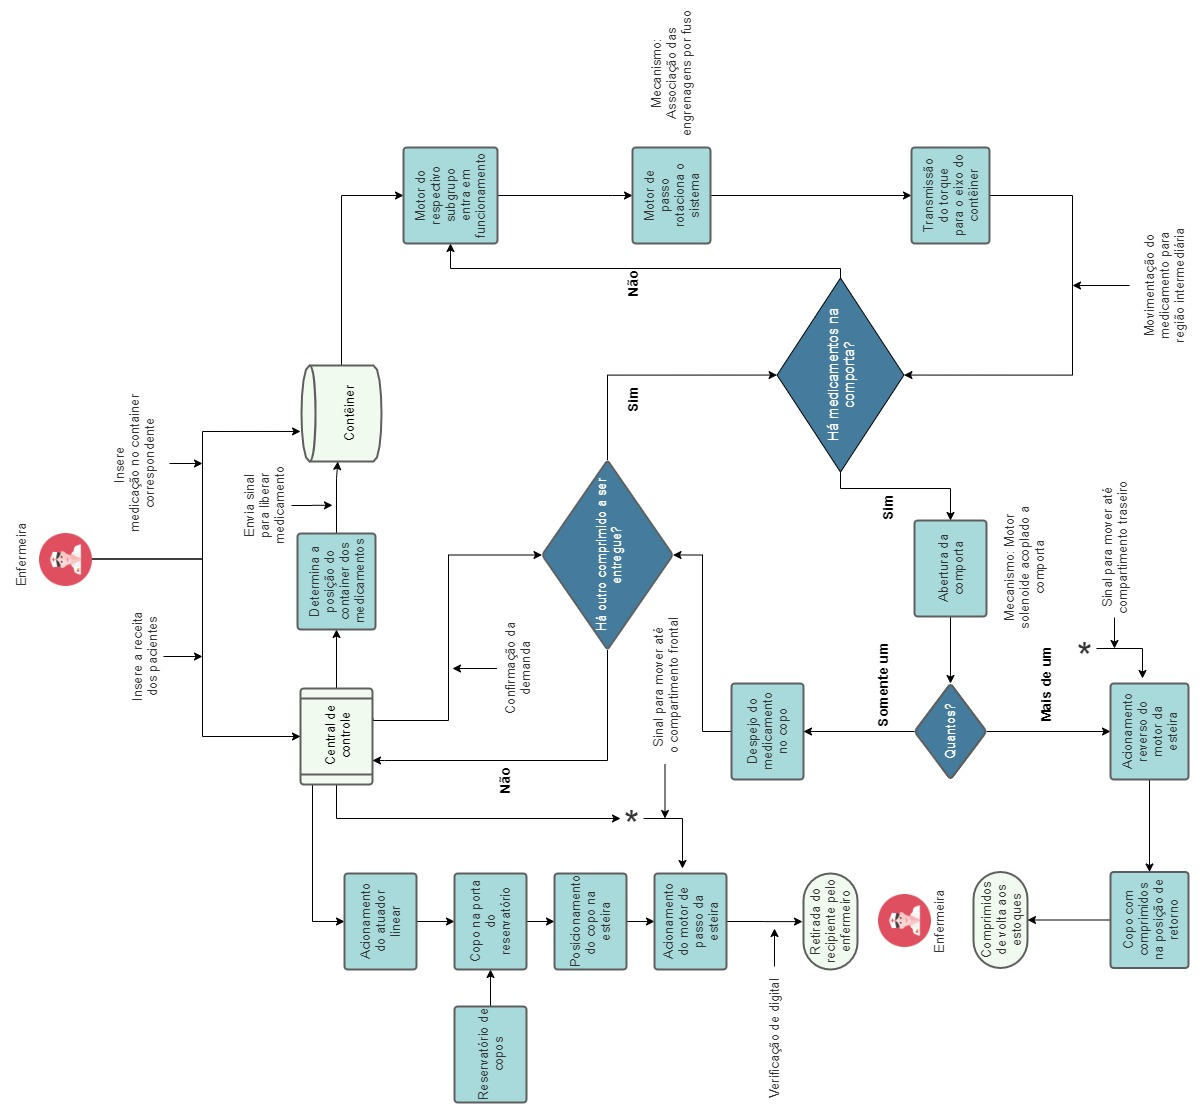
\includegraphics[width=1.15\textwidth, angle = -90]{figuras/estrutura/FEstrV35.jpg}
        \caption{Fluxograma de operação do Sistema Mecânico}
        \label{fig:FEst}
    \end{figure}

\paragraph*{O processo é iniciado:}

\begin{enumerate}
    \item[1.] Inserção de dados feita pelo enfermeiro do usuário e a respectiva entrada dos medicamentos no Contêiner.
    \item[2.] Determinação da posição dos contêiners dos medicamentos pela central de controle.
    \item[3.] Envio do sinal para liberar a medicação por demanda.
    \end{enumerate} 
   
% O conjunto abaixo entraria em ação após execução da etapa 3.
\paragraph*{O conjunto abaixo entraria em ação após execução da etapa 3:}

\begin{enumerate}
    \item [4.] Acionamento do micro atuador linear por demanda da central de controle.
    \item [5.] Posicionamento do copo no local de deposição dos medicamentos o e o recipiente adjacente (próximo copo) assume a posição inicial após o retorno do atuador linear para a posição de repouso.
    \item [6.] Pausa até a verificação de funcionamento dos motores de passo ser concluída.
\end{enumerate}
    
    % Enquanto a movimentação do copo pela esteira se conclui, a ação do sistema de seleção tem início:
\paragraph*{Enquanto a movimentação do copo pela esteira se conclui, a ação do sistema de seleção tem início:}

\begin{enumerate}
    \item[7.] Verificação da presença de medicamentos na região intermediária do sistema (anterior à comporta).
    \item[8.] Abertura da comporta do contêiner por motor solenóide.
    \item[9.] Verificação da quantidade de comprimidos despejados pelo sistema no recipiente do usuário (copo).
\end{enumerate}
   
    % Caso não seja detectada a presença do medicamento na região intermediária (parte  anterior à comporta), a sequência ocorre:
\paragraph*{Caso não seja detectada a presença do medicamento na região intermediária (parte  anterior à comporta), a sequência ocorre:}

\begin{enumerate}
    \item[10.] Início da operação do motor do subgrupo do contêiner selecionado.
    \item[11.] Motor de passo rotaciona o fuso.
    \item[12.] Transmissão do torque para os eixos dos contêiners por meio de engrenagens helicoidais.
    \item[13.] Posicionamento do remédio na região intermediária.
    \item[14.] Abertura da comporta do contêiner por motor solenóide.
    \item[15.] Checagem de sensores da queda dos medicamentos para repetição ou fim do ciclo de rotação.
    \item[16.] Verificação da quantidade de comprimidos despejados pelo sistema no recipiente do usuário (copo).
    \item[17.] Repetição do ciclo a partir da etapa 7 até que todos os comprimidos selecionados sejam entregues.
\end{enumerate}


    % Durante o processo de escolha dos medicamentos do paciente, a verificação irá traduzir na atuação da esteira como segue:
\paragraph*{Durante o processo de escolha dos medicamentos do paciente, a verificação irá traduzir na atuação da esteira como segue:}

\begin{enumerate}
    \item[18a.] A medicação é verificada e não há erros detectados pelos sensores.
    \item[19a.] Acionamento do motor de passo da esteira no sentido usual.
    \item[20a.] Operação da esteira até local de retirada do enfermeiro. 
    \item[21a.] Verificação de digital e abertura do compartimento frontal.
\end{enumerate}
   
\paragraph*{Caso seja identificada alguma falha:}

\begin{enumerate}
    \item[18b.] A medicação é verificada e erros são encontrados pelos sensores.
    \item[19b.] Acionamento reverso do motor da esteira.
    \item[20b.] Operação da esteira até o compartimento traseiro.
    \item[21b.] Despejo do copo no compartimento traseiro.
    \item[22b.] Medicação extra preparada para remoção pelo enfermeiro.
\end{enumerate}

\subsection{Escolha de Materiais}
No desenvolvimento de tecnologias médicas, a escolha dos materiais assume um papel de importância ainda mais relevante do que em outras soluções tecnológicas, pois os materiais nestes casos devem atender não somente aos requisitos de engenharia estrutural, mas também aos protocolos de segurança da saúde \cite{Steel_Group}.

Com o aumento das restrições de projeto, há uma diminuição da quantidade de materiais disponíveis para atender a solução, dessa forma, a escolha se torna mais limitada e responsável. Os materiais apresentados a seguir, tiveram sua escolha baseada em três segmentos gerais: segurança sanitária; propriedades de engenharia e custos.

\subparagraph*{$\bullet$ Aço Inoxidável 304} \hfill

O tipo de aço inox escolhido pertence a família dos austeníticos, o que significa que ele é composto basicamente por: ferro; cromo e níquel. Garantindo assim, uma alta resistência a oxidação, a corrosão, boa conformabilidade e boa soldabilidade \cite{Askeland_Wright_2019}. Além das vantagens apresentadas a cima, o aço inox 304, possui características essenciais para o setor da saúde:
\begin{itemize}
    \item []

    \begin{itemize}
        \item Superfície não porosa, o que proporciona uma diminuição do risco de contaminação por bactérias e vírus.
        \item Resistente a produtos químicos.
        \item Fácil higienização.
        \item Material não magnético. 
        \item Resistente ao Calor.
        \item Reciclável.
    \end{itemize}
\end{itemize}
    

\begin{table}[H]
    \centering
    \caption{Propriedades do Aço Inox 304.}
    \label{fig:PropAI}
    \begin{adjustbox}{max width = \textwidth}
        \begin{tabular}{|L{2cm}|C{2cm}|C{2cm}|C{2cm}|C{3cm}|C{3cm}|C{2.8cm}|C{2cm}|}
            \hline
            \rowcolor[HTML]{A8DADC}
            \textbf{Aço Inox} & \textbf{\%C} & \textbf{\%Cr} & \textbf{\%Ni} & \textbf{Limite de Resistencia (Mpa)} & \textbf{Limite de Escoamento (Mpa)} & \textbf{Alongamento (\%)} & \textbf{Condição}  \\ \hline
            
              304 & 0,08 & 19 & 10  & 517 & 207 & 30 & Encruado
             \\ \hline
            
        \end{tabular}
    \end{adjustbox}
\end{table}

\subparagraph*{$\bullet$ Aço-carbono 1020} \hfill

O material em questão foi escolhido por apresentar características técnicas e orçamentarias que contribuem para o sucesso do projeto. Seguindo \cite{Aco_1020_ensaio}, a quantidade de cementita apresentada na metalografia do aço 1020 proporciona ótima resistência à traç{\~a}o e propriedades mecânicas para as mais diversas aplicações industriais. Serão utilizados tanto aço de classificação SAE como da classificação AISI, não por requisitos estruturais, mas pela disponibilidade no mercado e pelo escopo de custos do projeto. Seguem os fatores responsáveis pela escolha do aço-carbono 1020:

\begin{itemize}
    \item []
    \begin{itemize}
        \item Boa conformabilidade.
        \item Boa soldabilidade.
        \item Custo-benefício.
    \end{itemize}
\end{itemize}

\begin{table}[H]
    \centering
    \caption{Propriedades do Aço 1020.}
    \label{fig:PropA1020}
    \begin{adjustbox}{max width = \textwidth}
        \begin{tabular}{|L{2cm}|C{2cm}|C{2cm}|C{2cm}|C{3cm}|C{3cm}|C{2.8cm}|C{2cm}|}
            \hline
            \rowcolor[HTML]{A8DADC}
            \textbf{Aço } & \textbf{\%C} & \textbf{\%Mn} & \textbf{Limite de Resistencia (Mpa)} & \textbf{Limite de Escoamento (Mpa)} & \textbf{Alongamento (\%)}\\ \hline
            
              1020 & 0,18-023 & 0,30-0,60 & 450  & 330 & 36
             \\ \hline
            
        \end{tabular}
    \end{adjustbox}
\end{table}
\subparagraph*{$\bullet$ Polipropileno (PP)} \hfill

O presente polímero termoplástico foi escolhido depois de se assumir requisitos essenciais para o sucesso do projeto e buscar o material que mais se adequasse a essas exigências. Segundo \cite{PP_Recycle}, o polipropileno é muito utilizado na indústria farmace{\'u}tica para frascos de prescriç{\~a}o, recipientes de medicamentos, tanto ovais como cilindricos e quadrados, e também para fechamento de recipientes. A seguir são listados os fatores responsáveis pela escolha do polipropileno: 

\begin{itemize}
    \item[ ]
    \begin{itemize}
        \item Baixo custo.
        \item Reciclável.
        \item Comportamento mecânico. 
        \item Comportamento plástico.
        \item Comportamento dúctil.
        \item Atoxidade
        \item Baixa absorção de umidade.
        \item Resistência química.
        \item Resinas com baixo potencial de contaminação
    \end{itemize}
\end{itemize}

\begin{table}[H]
    \centering
    \caption{Propriedades do Polipropileno (PP).}
    \label{fig:PropPP}
    \begin{adjustbox}{max width = \textwidth}
        \begin{tabular}{|L{2cm}|C{3cm}|C{2.8cm}|C{2cm}|C{2.5cm}|C{2.5cm}|}
            \hline
            \rowcolor[HTML]{A8DADC}
            \textbf{Polímero} & \textbf{Resistência a tração na ruptura (Mpa)} & \textbf{Alongamento } & \textbf{Módulo Elástico (Mpa)} & \textbf{Massa Específica (g/cm3)} & \textbf{Resistencia ao Impacto (J/cm)} \\ \hline
            
              Polipropileno (PP) & 41 & 700 & 1517  & 0,90 & 0,50
             \\ \hline
        \end{tabular}
    \end{adjustbox}
\end{table}

\subparagraph*{$\bullet$ Nylon (NY)} \hfill

A escolha do Nylon para o projeto se deu pela sua facilidade de manipulação e custo operacional. Segundo \cite{Imp3D_Polimeros},o Nylon é um plástico de baixo custo, forte, leve e flexível, que possui propriedades coo estabilidade dimensional, boa resistência ao impacto sem entalhe e excelente resistência química. Ele é muito utilizado tanto para Impressão 3D de componentes, como para extrusão e injeção de peças.

\subparagraph*{$\bullet$ ABS} \hfill

Outro material também utilizado no projeto é o ABS, um copolímero utilizado na impressão 3D que traz um alto grau de detalhamento para as peças. Segundo \cite{Imp3D_Polimeros}, o ABS é superior ao PLA em relação à propriedades mecânicas, é durável, forte e é considerado leve. Suporta altas temperaturas e é um dos termoplásticos mais baratos no mercado de filamentos. 

\subparagraph*{$\bullet$ Silicone} \hfill

O silicone também possui papel fundamental neste projeto, pela sua alta maleabilidade de uso. Segundo \cite{Silicone_estudo}, o silicone é utilizado para resistir a altas temperaturas, resistência às imtemperies, biocompatibilidade, além de alta estabilidade, baixa tensão superficial e falta de toxicidade, o que permite sua utilização com medicamentos.


\section{Solução de Eletrônica}

A solução de eletrônica será dividida em 3 sistemas: Módulo de Medição, Central de Controle e Sistema de Acionamento de Atuadores. Consequentemente, os sistemas possuem grande dependência entre si.

\subsection{Módulo de Medição}

O módulo de medição é o sistema com funcionalidade de realizar a captura de dados de interesse para uso no controle e automação do dispositivo. Sendo assim, se trata de um sistema micro-controlado pela central de controle conectado a vários componentes de detecção e medição. Dessa forma, os componentes de detecção e medição foram filtrados a partir dos requisitos levantados, disponibilidade no Brasil, apresentarem custos acessíveis e escala de medição compatível com a aplicação.



% \begin{itemize}
    % \item Sensor de Temperatura e Umidade
    \subparagraph*{$\bullet$ Sensor de Temperatura e Umidade} \hfill
    
    O uso do sensores de temperatura e de umidade foi baseado na necessidade do monitoramento constantes das variáveis de temperatura e umidade relativa dentro do dispositivo. A maioria dos medicamentos sólidos precisa estar em uma faixa de temperatura específica e umidade relativa para não alterar as propriedades químicas. Caso contrário, existe a diminuição da eficácia dos medicamentos armazenados em condições não recomendadas pelo fabricante. 
    
    Para seleção dos componentes foram priorizados sensores com mais de uma funcionalidade, logo, sensores de temperatura e umidade integrados. Sendo assim, a faixa de valores para a conservação de medicamentos sólidos está entre 15 $^\circ$C a 30 $^\circ$C e a escala de umidade relativa de 40\% e 70\% \cite{Pinto_2016}. Logo foi selecionado o sensor \textbf{HTU21D}, figura \ref{fig:sensor_temp_umidade}, com as seguintes características:

    \begin{itemize}
    \item[ ]
        \begin{itemize}
            \item Alimentação: 1,5V a 3,6V;
            \item Faixa de medição da umidade: 0-100\% RH;
            \item Faixa de temperatura de medição: -40 a 105 $^\circ$C;
            \item Precisão da umidade (10\% RH a 95\% RH):  2\% RH.
            \item Comunicação: I$^2$C;
        \end{itemize}
    \end{itemize}

    \begin{figure}[H]
        \centering
        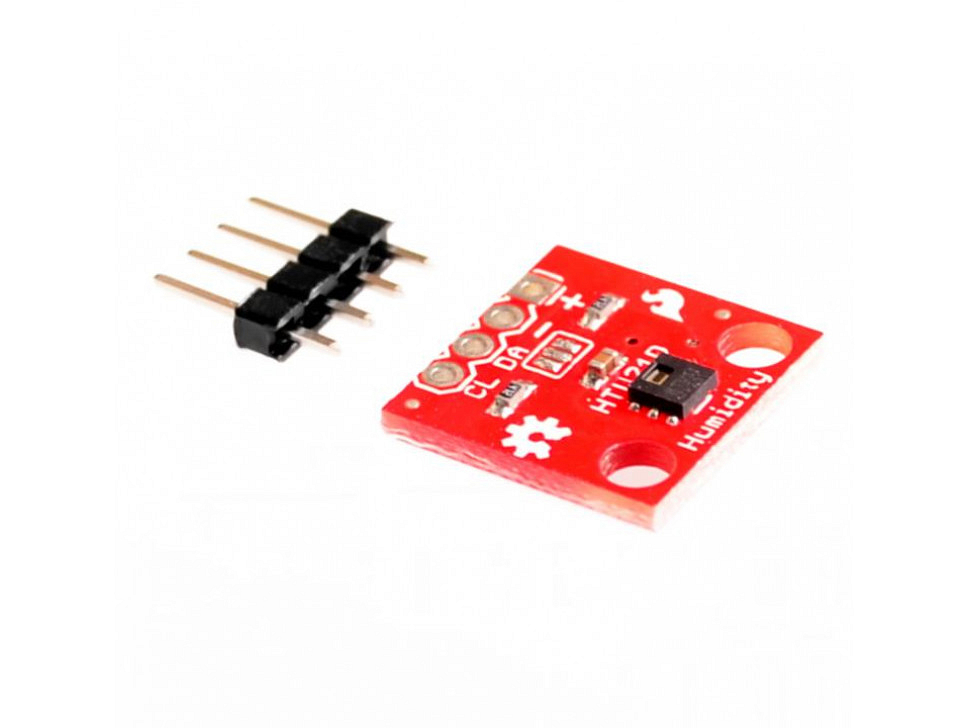
\includegraphics[width=0.3\textwidth]{figuras/sensor_temp_umi.jpg}
        \caption{Sensor de Temperatura e Umidade}
        \label{fig:sensor_temp_umidade}
    \end{figure}

    % \item Interruptor
    \subparagraph*{$\bullet$ Interruptor} \hfill
    
    O uso de interruptores se deve a necessidade de detectar o trancamento da compartimento frontal, por onde ocorre a passagem dos copos com medicamento do dispositivo, e da compartimento traseiro, por onde ocorre o acesso aos contêineres de estoque com medicamento. Da mesma forma é utilizado para detectar se os contêineres individuais, onde são colocados os medicamentos, foram encaixados corretamente.
    
    
    Com base na aplicação levantada foram selecionados, de forma qualitativa, os interruptores do tipo \textit{micro switch}. Seu uso é ideal para as aplicações descritas devido a direção em que o interruptor é ativado, o mecanismo relacionado ao acoplamento e desacoplamento e a força mínima necessária para a ativação. 
    
    \begin{figure}[H]
        \centering
        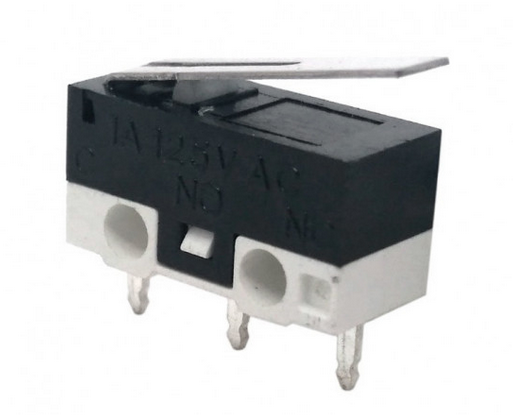
\includegraphics[width=0.2\textwidth]{figuras/microswitch.png}
        \caption{Interruptor tipo \textit{Micro Switch}}
        \label{fig:micro_switch}
    \end{figure}
    
    % Chave Micro Switch KW10-B com Haste - Preço: 0,80 cada - https://www.baudaeletronica.com.br/chave-micro-switch-kw10-b-com-haste.html
    % Necessario 2 (cada porta) + 25 (cada container) = 27 -> 27*0,80 = 21,60
    
    % \item Sensor Fotoelétrico
    \subparagraph*{$\bullet$ Sensor Fotoelétrico} \hfill
    
    Os sensores fotoelétricos trabalham com emissão e recepção de luz e são ideais para aplicações onde faz-se necessário a detecção de objetos sem o contato físico. Dessa forma, estes sensores serão utilizados para detectar a passagem do medicamento sólido tanto na saída das comportas quanto no final da zona de transição. Além do mais, também será utilizado esse sensor para as seguintes detecções: presença do copo no reservatórios de copos, identificação da presença do copo em local predeterminado para recebimento de medicamentos, passagem do copo com medicamentos errados para o compartimento traseiro e passagem do copo para o compartimento frontal.
    
    Assim, optou-se pela utilização do sensor de barreira (foto interruptor), o qual o emissor e o receptor são instalados frente a frente para permitir que a luz do emissor entre no receptor. Logo, quando um objeto passa entre o emissor e o receptor a luz que entra no receptor é interrompida ou reduzida e assim é possível detectar um objeto \cite{amron_photo_sensors}.
    
    
    \begin{figure}[H]
        \centering
        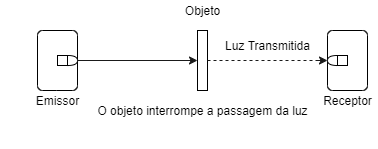
\includegraphics[width=0.5\textwidth]{figuras/sensor_infra.png}
        \caption{Sensores de Barreira}
        \label{fig:sensor_infra}
    \end{figure}
    
    Por se tratar de um sensor de simples implementação, o subgrupo optou em fazer a implementação utilizando: um \textit{LED} emissor de infravermelho (\textbf{IR333C}), um fototransistor receptor de infravermelho (\textbf{PT333-3B}) e circuito comparador (\textbf{LM393}).
    
    % \item Sensor de Biometria
    \subparagraph*{$\bullet$ Sensor de Biometria} \hfill
    
    O sensor de biometria é utilizado para autenticação de usuários nos mais diversos produtos no mercado. O seu funcionamento se baseia na captura da digital do usuário por meio de uma imagem que posteriormente terá suas características únicas extraídas e comparadas com um banco de dados de digitais cadastradas. 
    
    Dessa forma foi escolhido o sensor óptico de digitais \textbf{FY50}, figura \ref{fig:sensor_biometria}, por ser o mais comum no mercado e possuir um sistema  validado para obtenção de digitais. Esse sensor tem a funcionalidade de legitimar o funcionário da clínica geriátrica e permitir realizar funções que necessitam de autenticação. Assim, esse sensor é empregado para liberar o compartimento frontal/traseiro para a retirada da dose medicamentosa do dispensador e realizar o abastecimento do estoque de medicamentos.
    
    \begin{figure}[H]
        \centering
        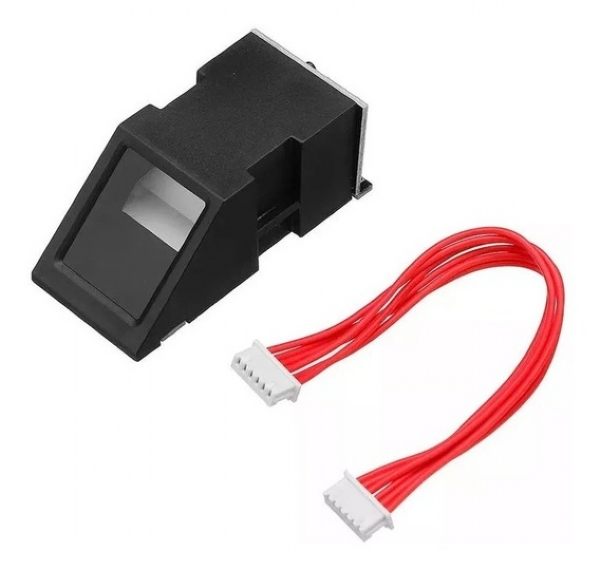
\includegraphics[width=0.2\textwidth]{figuras/sensor_biometria.jpg}
        \caption{Sensor FY50}
        \label{fig:sensor_biometria}
    \end{figure}
    
    % \item Sensor de Leitura RFID
    \subparagraph*{$\bullet$ Sensor de Leitura RFID} \hfill
    
    O sensor de identificação por radiofrequência (RFID) utiliza um sistema de energização sem fio de etiquetas RFID para obtenção de dados armazenados nelas. Dessa forma, é utilizada uma antena que realiza a energização e captação desses dados numa frequência de 13.56 MHz, que posteriormente são decodificados e enviados por meio do protocolo I$^2$C para central de controle. 
    
    O uso do sensor RFID foi pensado para identificar os copos utilizados para armazenar as doses de medicamentos. Desse modo, sua identificação é necessária para determinar o copo que está recebendo a medicação. Para realizar a identificação e logística de distribuição de medicamentos para os pacientes cada copo tem cores únicas para evitar ministração de doses medicamentosas para pacientes errados. 
    
    Com o posicionamento da etiqueta RFID na parte inferior do copo é possível ler sua identificação independentemente da face virada para o sensor. Uma vez que o sensor será posicionado entre as placas da esteira e o sensor poder identificar etiquetas RFID com uma distância determinada dependendo da antena utilizada. Como as placas da esteira utilizada são feitas de plástico não ocorrerá problemas em relação a interferência na posição onde foi definido. 
    
    O modelo \textbf{PN532}, figura \ref{fig:sensor_RFID}, foi escolhido pela sua capacidade de distância de ativação das etiquetas chegar à 50mm e sua antena pode ser modificada e direcionada para atender as necessidades de dimensionamento da máquina.
    
    \begin{figure}[H]
        \centering
        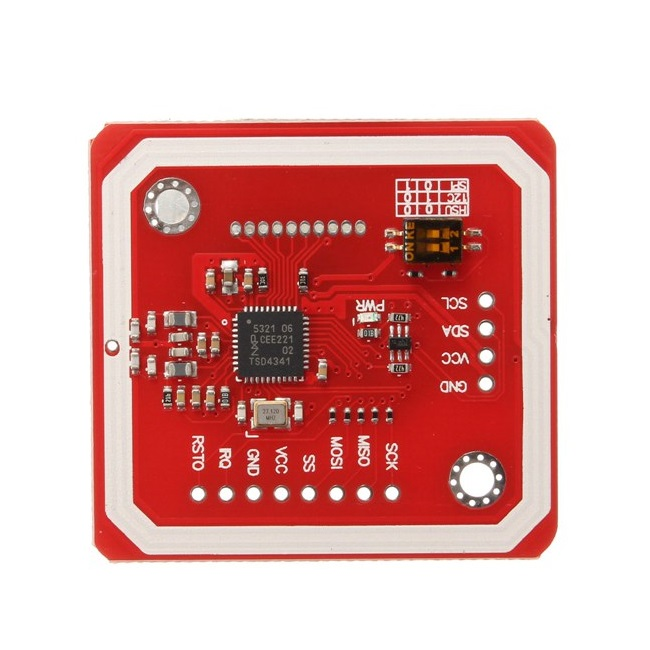
\includegraphics[width=0.2\textwidth]{figuras/sensor_RFID.jpg}
        \caption{Sensor PN532}
        \label{fig:sensor_RFID}
    \end{figure}
    
    
    % \item Câmera para Processamento de Imagens
    \subparagraph*{$\bullet$ Câmera para Processamento de Imagens} \hfill
    
    Atualmente câmeras estão presentes no dia-a-dia da população mundial, porém ainda mais presentes na automatização de processos industriais e verificação de qualidade por meio do processamento de imagens. Dessa forma, o uso de uma câmera foi escolhida para realizar a captação visual dos comprimidos. Posteriormente, a partir do  processamento dessas imagens, serão extraídas as características dos comprimidos, sendo possível identificar a quantidade e classificar o tipo de medicamento no copo de forma eficiente e confiável.
    
    A câmera escolhida foi a \textbf{OV5647}, figura \ref{fig:camera_process}, por apresentar sensor com capacidade de gerar imagens de até 2592x1944 pixeis e preço acessível no Brasil. Ela utiliza o protocolo CSI para transmitir dados, sendo um padrão muito utilizado na indústria facilitando assim sua integração.
    
    \begin{figure}[H]
        \centering
        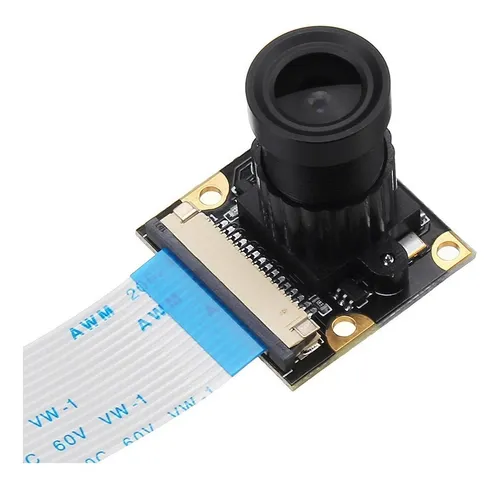
\includegraphics[width=0.2\textwidth]{figuras/OV5647.png}
        \caption{Câmera OV5647 - 5MP}
        \label{fig:camera_process}
    \end{figure}
    
    Para o processamento será aplicada uma técnica que consiste em detectar as bordas dos medicamentos. Com isso é criado máscaras binárias para cada comprimido identificado, isolando o comprimido e extraindo características do mesmo, como por exemplo cor e formato.
    
    Após isso, será utilizado um classificador \textit{SVM}, treinado com uma biblioteca de imagens de comprimidos que tiveram as mesmas características extraídas. Sendo assim cruzados os dados dos comprimidos que eram previstos no copo com os dados do classificador SVM, obtendo resultado positivo caso seja verificado que a dose está correta. 
    
    O classificador \textit{SVM} foi escolhido por ter solução determinística, não possuindo viés de treinamento e não consumindo muitos recursos do sistema embarcado. 
% \end{itemize}

\subsection{Sistema de Acionamento de Atuadores}
     
    O sistema de acionamento de atuadores tem a funcionalidade de controlar os atuadores contidos no dispositivo. Sendo assim, o sistema de acionamento de atuadores  trata-se de um sistema micro-controlado pela central de controle e são utilizados \textit{drivers} que controlam os atuadores do dispositivo. Sendo estes: motor DC, atuador, motores de passo, solenoides para os contêineres e as mini travas elétricas solenóides em cada compartimento de acesso no sistema. 

% \begin{itemize}
%    \item Fechaduras
    % \item Drivers
    \subparagraph*{$\bullet$ Drivers} \hfill
    
    Os \textit{drivers} dos atuadores são módulos projetados para prover a potência de atuação e a interação com o controle de forma simplificada. Eles convertem comandos por meio de portas lógicas em potência controlada para os atuadores. Dessa forma, tornam possível o controle automático de ações de movimento. 
    
    O \textit{driver} escolhido para os motores de passo é o CI \textbf{TB6560} pois possui uma corrente de até 3A e utiliza opto-acopladores em sua entrada de sinal, o que diminui o ruído proveniente do motor de passo de chegar até a central de controle.
    
    O \textit{driver} escolhido para as solenoides é o \textbf{L295} por possuir 2 canais com corrente máxima de até 2A e suas configurações possibilitam a utilização de tensões da porta lógica do microcontrolador para controle. Além de possuir 2 fontes de tensão independentes para periféricos com tensões acima de 5V.
    
    O \textit{driver} escolhido para o motor DC é o \textbf{L298}, seu controle é baseado na ponte H. Essa estrutura de eletrônica de potência permite a manipulação da tensão da fonte no motor por meio de chaveamento, dessa forma, é possível controlar a velocidade do motor. Para o chaveamento será utilizado o controle por modulação de pulso (\textit{PWM}), presente no microcontrolador. Essa tecnologia varia o tempo de permanência do sinal lógico em baixo e alto, isso acarreta uma resposta que simula uma variação de intensidade de tensão, porém variando apenas o tempo que o sinal está ligado.  
    
    
    % \item Isolamento
    \subparagraph*{$\bullet$ Isolamento} \hfill
    %% Escrever texto básico para usando optoacopladores
    
    A natureza dos atuadores gera ruídos de tensão e corrente que devem ser tratados, uma vez que, caso esse ruído chegue ao sistema de controle existe a possibilidade de causar mal funcionamento das funções de todos os circuitos presentes. Portanto, deve-se isolar o sistema de atuadores do sistema de controle. Para isso são utilizados opto-acopladores, que isolam o sistema transferindo sinais por meio de \textit{LEDs} emissores e receptores.
    
% \end{itemize}

\subsection{Central de Controle}

A central de controle é o sistema que irá realizar tanto a análise dos dados coletados no módulo de medição quanto o controle do sistema de atuadores do dispositivo. Bem como é por onde se recebe e se envia comandos no \textit{Backend} - nome que representa a parte da arquitetura de software que interage com a central de controle. 

O principal componente da central de controle é o microprocessador embarcado. Adicionalmente também temos aspectos funcionais para os usuários que interagem com o dispositivo. Esta interação é feita pelo subsistema denominado módulo de visualização.

\newpage
% \begin{itemize}
%     \item Microprocessadores
    \subparagraph*{$\bullet$ Microprocessadores}  \hfill
    
    A adoção de microprocessadores é bastante comum atualmente em implementações de sistemas embarcados nas mais diversas aplicações. Em especial temos diversos fabricantes que implementaram sistemas usando microprocessadores que tem suporte a vários Sistemas Operacionais (SO) diferentes e incluem uma interface de entradas e saídas digitais com propósito geral, sendo denominadas como computadores de placa única (\textit{Single Board Computers} - SBCs). Alguns exemplos comuns no mercado são as placas \textit{Raspberry's Pi} desenvolvidas pela \textit{Raspberry Pi Foundation}, placas Tinker da ASUS, placas BeagleBoards da Texas Instruments e as placas NVIDIA Jetson da NVIDIA. 
    
    O sistema eletrônico desempenha várias funções que necessitam do uso de processos com maior demanda de processamento e memória, como: Processamento de imagens; interface gráfica do módulo de visualização; Captura de dados de múltiplos sensores; Controle refinado dos atuadores.
    
    Assim como, também é necessário o suporte a protocolos de comunicação como I$^2$C, \textit{SPI}, \textit{UART} e \textit{CSI} além de um sistema operacional com suporte as ferramentas e algoritmos de comunicação com as arquiteturas usadas na área de Software.
    
    Após uma análise de vários modelos comparando principalmente os componentes integrados como processador central (CPU), processador gráfico (GPU), tipo de memória RAM, quantidade de memória RAM, periféricos embarcados (tipo USB, módulo Wi/Fi, internet) e o preço relativo praticado em fornecedores no Brasil foi escolhido a \textbf{Raspberry 4 B} com \textbf{4GB DDR4}.
    
    
    % \item Módulo de Visualização
    \subparagraph*{$\bullet$ Módulo de Visualização} \hfill
    
    O módulo de visualização é o subsistema onde o usuário poderá visualizar algumas informações úteis de funcionamento e gestão do dispositivo e interagir com essa interface usando as teclas como meio de interação. Nele estão contidos um visor e um teclado para interface com o usuário.


    % \begin{itemize}
    %     \item Visor 
        \subparagraph*{}$\bullet$ Visor \hfill
        
        Existem diversas tecnologias de tela disponíveis no mercado que podem ser utilizadas no projeto. Para delimitação da tela foi levado em consideração compatibilidade do protocolo de comunicação com sistema microprocessado escolhido, tamanho da tela, tecnologia de tela para visualização nas cores RGB e preço relativo. Sendo assim foi escolhido a tela tipo LCD TFT de 3,2” com as seguintes características:
        
        \vspace{-0.2cm}
        \begin{itemize}
            \item[ ] 
            \begin{itemize}
            \item \textbf{\textit{Display}:} Tipo LCD TFT 3.2" 
            \item \textbf{Controlador:} ILI9341
            \item \textbf{Resolução:} 240x320 pixels
            \item \textbf{Dimensões da tela:} 48.60 x 64.80 mm
            \item \textbf{Interface:} SPI
            \end{itemize}
        \end{itemize}
        
        \vspace{-0.2cm}
        \begin{figure}[H]
            \centering
            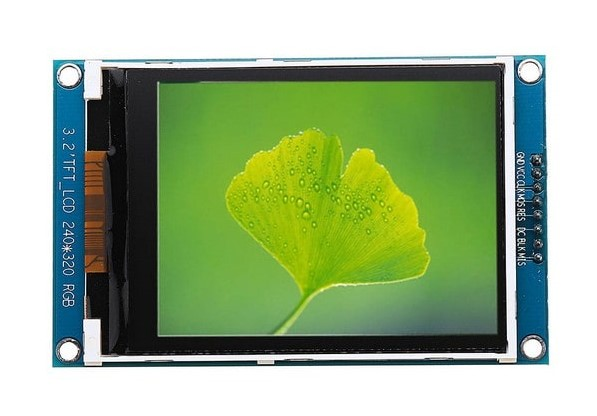
\includegraphics[width=0.5\textwidth]{figuras/Display-LCD-TFT-3.2-240x320-6.jpg}
            \caption{Visor tipo LCD TFT}
            \label{fig:display_lcd}
        \end{figure}
        
        
        % \item Teclado
        \subparagraph*{}$\bullet$ Teclado \hfill
        
        
        A utilização de uma matriz de botões é necessária para o usuário do dispositivo poder interagir com os menus de opções disponíveis na tela de visualização. Neste caso foi preferível o uso de botões para manter as opções de interação o mais simples possível para o usuário final e para utilizar menos processamento do sistema microprocessado.
        
        
        Sendo assim será usado uma configuração de arquitetura chamada de matriz de botões, especificamente uma solução comercial \textit{AdKeypad} com 5 botões como foto na figura \ref{fig:keypad_ft}.
        
        \begin{figure}[H]
          \centering
          \begin{minipage}[b]{0.3\textwidth}
            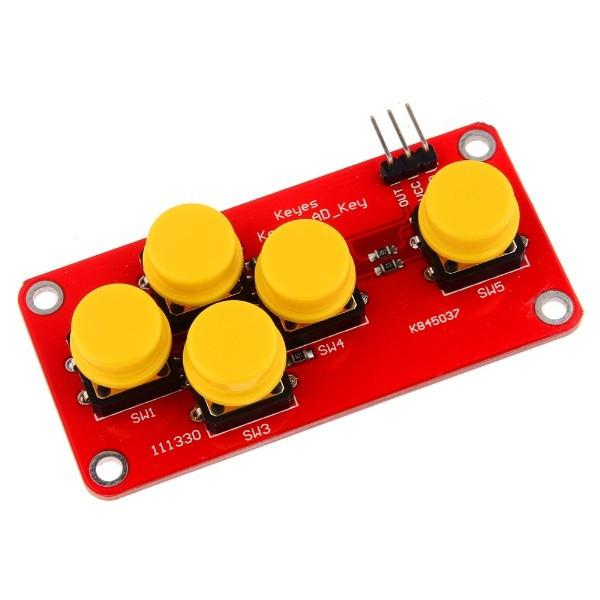
\includegraphics[width=\textwidth]{figuras/adkeypad.jpg}
            \caption{\textit{AdKeypad} com 5 botões}
            \label{fig:keypad_ft}
          \end{minipage}
          \hspace{2cm}
          \begin{minipage}[b]{0.3\textwidth}
            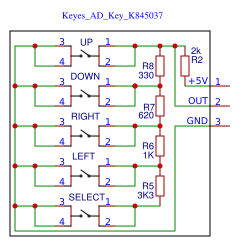
\includegraphics[width=\textwidth]{figuras/adkeypad_schematic.png}
            \caption{Esquemático \textit{AdKeypad}}
            \label{fig:keypad_esq}
          \end{minipage}
        \end{figure}
        
        Conforme o esquemático, o qual representa como foi implementado a solução escolhida, na figura \ref{fig:keypad_esq}, pode-se observar que existe apenas um pino de dados (2) para esse teclado. Seu funcionamento se baseia em um circuito com várias divisões de tensão. A central de controle irá interpretar qual botão foi pressionado a partir do sinal digital resultante da conversão analógica digital da tensão de saída no pino de dados (2). Essa conversão é realizada em um micro controlador, na qual o pino (2) de dados será conectado a uns dos pinos A/D de um dos microcontroladores que são usados no módulo de medição. 
    % \end{itemize}
    
    % \item Microcontroladores
    \subparagraph*{$\bullet$ Microcontroladores} \hfill
    
    Os microcontroladores são utilizados nas mais diversas aplicações de controle e automação. Assim, os microcontroladores possuem os itens essenciais de processamento, aliados a periféricos abundantes para entradas e saídas de dados com um  baixo custo, possibilitam o desenvolvimento de sistemas robustos e escaláveis.
    
    Em nosso projeto, os microcontroladores serão utilizados para direcionar dados do módulo de medição para o sistema microprocessado e o mesmo enviar dados de controle para o sistema de acionamento de atuadores. Dessa forma, a informação presente nos microcontroladores será direcionada para o barramento de dados por meio de protocolo I$^2$C, principal de protocolo de comunicação com a sistema microprocessado.
    
    O microcontrolador escolhido foi o \textbf{PIC16F677} por possuir 16 portas IO e comunicação I$^2$C. Sua interação será diretamente vinculada ao módulo de medição e ao sistema de acionamento dos atuadores. Para evitar qualquer ruído inerente dos atuadores serão usados microcontroladores exclusivos tanto para o sistema de acionamento dos atuadores quanto para o módulo de medição. Desse modo, é garantida uma integridade dos valores medidos dos sensores no módulo de medição.
    
    Para administrar todos os sensores fotoelétricos nas comportas do solenoide de cada contêiner de medicamento será utilizado o CI de modelo \textbf{CD4051} no modo multiplexador ligado diretamente ao microcontrolador para diminuir a quantidade de portas necessárias para esses sensores. Como a operação dos contêineres será restrita a um por vez, não é necessário haver a medição simultânea dos sensores fotoelétricos presentes em sua estrutura, tornando a multiplexação uma forma eficiente de obtenção de dados.
    
    Esses dados se apresentam como um nível de tensão com dois possíveis valores, 0V para quando há um comprimido presente ou 5V quando não há. Então a saída do multiplexador será lida por uma porta lógica presente no microcontrolador. O controle dos multiplexadores será feito por meio de três portas lógicas para cada um, que selecionarão o sensor requerido por meio de alternação dos níveis lógicos nelas.
    
    Para administrar os solenoides também será utilizado o CI de modelo \textbf{CD4051}, porém no modo demultiplexador. Dessa forma é possível escolher em qual solenoide o sinal do microcontrolador será direcionado, o que diminui a quantidade de portas utilizadas. Como os atuadores não serão utilizados paralelamente, a demultiplexação do sinal de controle torna a manipulação do sistema de atuadores mais eficiente e também reduz o pico máximo de corrente de todo o sistema.
    
% \end{itemize}

    
\subsection{Arquitetura Inicial de Eletrônica}

\begin{figure}[H]
    \centering
    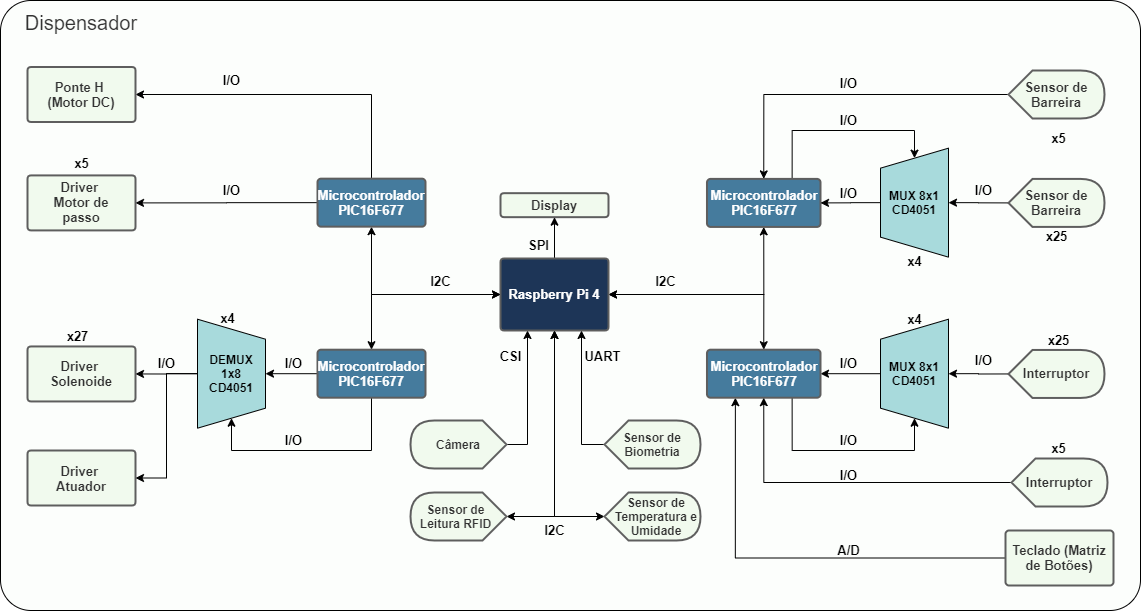
\includegraphics[width=\textwidth]{figuras/fluxograma_eletronica.png}
    \caption{Arquitetura Inicial de Eletrônica}
    \label{fig:fluxograma_eletronica}
\end{figure}
    
    
\section{Solução de Energia}
\label{Solução_energia}
% Cada frente deve adc os subtópicos que acharem pertinentes

O escopo da solução energética do projeto envolve a implementação de uma fonte de alimentação principal, uma fonte de alimentação alternativa e um sistema eletromecânico. Todos esses componentes serão ocultados do campo de visão do usuário. Os objetivos da solução envolvem alcançar um custo reduzido, alta eficiência, robustez e compactação da estrutura. A configuração da solução da alimentação do sistema está representada no diagrama de blocos simplificado da figura \ref{fig:energia_alimentacao}.

\begin{figure}[H]
    \centering
    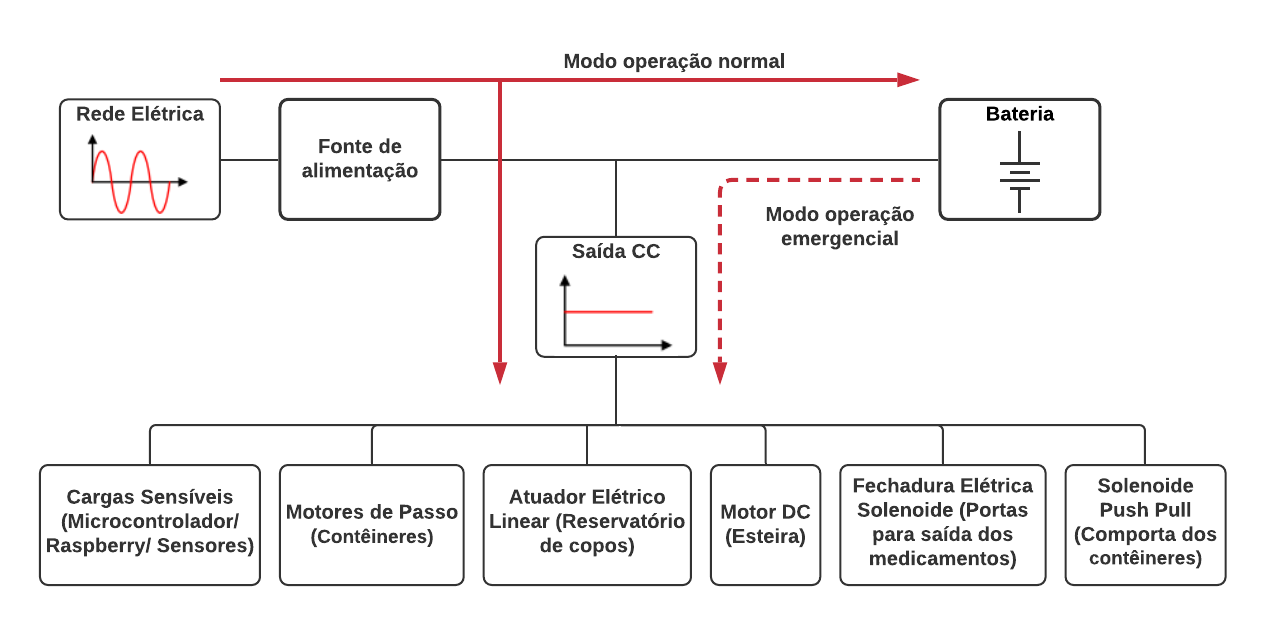
\includegraphics[width=1\textwidth]{figuras/Alimentação.png}
    \caption{Esquema do sistema de alimentação proposto.}
    \label{fig:energia_alimentacao}
\end{figure}

A carga do projeto será atendida de duas maneiras, considerando dois modos de operação: pela fonte de alimentação, quando houver energia elétrica na rede, e por uma fonte de alimentação alternativa, cuja função será atuar como uma fonte auxiliar/secundária que assegurará a ininterruptibilidade no provimento de energia em casos de falha da energia proveniente da rede primária.

O dimensionamento das duas fontes de alimentação será determinado principalmente pelo sistema embarcado e motores que atendam ao sistema de operação, e levará em conta sua distribuição espacial no equipamento. A tabela \ref{fig:energia_carga} contém o levantamento prévio da carga do sistema.

%A configuração contará com um sistema de proteção contra curto-circuito, sobrecarga, sobretensão, baixa tensão e ligação inversa da bateria.
 
\begin{table}[htb]
    \centering
    \caption{Levantamento prévio da carga do projeto.}
    \label{fig:energia_carga}
    \begin{adjustbox}{max width = \textwidth}
        \begin{tabular}{|L{5cm}|C{2cm}|C{2cm}|C{2cm}|C{2cm}|C{2cm}|}
            \hline
            \rowcolor[HTML]{A8DADC}
            \textbf{Equipamento} & \textbf{Quant. (unid.)} & \textbf{Tensão (V)} & \textbf{Corrente (A)} & \textbf{Potência (W)} \\ \hline
            Sensor de Temperatura e Umidade & 1	 & 3 & 0,0005 & 0,0015
            \\ \hline
           %   Sensor Fotoelétrico Emissor & 30	 & 3,3 & 0,1 & 9,9
         %   \\ \hline
              Sensor Fotoelétrico & 30	 & 3,3 & 0,1 & 9,9
             \\ \hline
             Sensor de Biometria & 1 & 3,6 & 0,12 & 0,432
             \\ \hline
             Sensor de Leitor RFID & 1	 & 3,3 & 0,025 & 0,0825
             \\ \hline
              Raspberry Pi 4 & 1 & 5 & 3 & 8
             \\ \hline
               Microcontrolador & 4 & 5 & 0,025 & 0,5
             \\ \hline
               Display & 1 & 3,3 & 0,001 & 0,0033
             \\ \hline
               Câmera & 1 & 3,3 & 0,2 & 0,66
             \\ \hline
            %  Teclado & 1 & X & X & X
            % \\ \hline
            %  Cls Mux/Demux & 12 & 5 & 0,000001 & 
            % \\ \hline
              Fechadura Elétrica Solenoide & 2 & 12 & 0,5 & 12
             \\ \hline
              Motor de Passo & 5 & 3,36 & 2,8 & 47,04
             \\ \hline
              Eletroímã Solenoide elétrico - atuador Push Pull & 25 & 5 & 1,12 & 140
             \\ \hline
                Motor DC & 1 & 4,5 & 1,2 & 5,4
             \\ \hline
                 Atuador Linear Elétrico & 1 & 12 & 2 & 24
             \\ \hline
               Driver para Motor de Passo & 5 & 12 & 3 & 180
             \\ \hline
                Driver L295 & 26 & 5 & 2 & 260
             \\ \hline
                  Driver Ponte H & 1 & 5 & 2 & 10
             \\ \hline
             \rowcolor[HTML]{F1FAEE}
             \multicolumn{4}{|l|}{\cellcolor[HTML]{F1FAEE}Total} & 698,02 \\
             \hline
        \end{tabular}
    \end{adjustbox}
\end{table}

A potência instalada do equipamento é igual a 698,02 W. A fonte de alimentação e a fonte auxiliar deverão ser dimensionadas com base na corrente total e no potencial de falha do pior caso. Portanto, serão considerados os seguintes cenários representados na tabela \ref{fig:energia_cenarios}. 

\begin{table}[H]
    \centering
    \caption{Cenários considerados para o dimensionamento dos sistemas de alimentação.}
    \label{fig:energia_cenarios}
    \begin{adjustbox}{max width = \textwidth}
        \begin{tabular}{|L{5cm}|C{2cm}|C{2cm}|C{2cm}|C{2cm}|C{2cm}|}
            \hline
            \rowcolor[HTML]{A8DADC}
            \textbf{Equipamento} & \textbf{Cenário 1} & \textbf{Cenário 2} & \textbf{Cenário 3} & \textbf{Cenário 4} \\ \hline
            Sensor de Temperatura e Umidade & x1 & x1 & x1 & x1
            \\ \hline
           %   Sensor Fotoelétrico Emissor & 30	 & 3,3 & 0,1 & 9,9
         %   \\ \hline
              Sensor Fotoelétrico & x30	 & x5 & x5 & x5
             \\ \hline
             Sensor de Biometria &  x1	 & x1 & x1 & x1
             \\ \hline
             Sensor de Leitor RFID & x1	 & x1  & x1 & x1
             \\ \hline
              Raspberry Pi 4 & x1 & x1 & x1 & x1
             \\ \hline
               Microcontrolador & x4 & x4 & x3 & x4
             \\ \hline
               Display & x1	 & x1 & x1 & x1
             \\ \hline
               Câmera & x1 & x1 & x1 & x1
             \\ \hline
            %  Teclado & 1 & X & X & X
            % \\ \hline
            %  Cls Mux/Demux & 12 & 5 & 0,000001 & 
            % \\ \hline
              Fechadura Elétrica Solenoide & x2	 & x2 & - & -
             \\ \hline
              Motor de Passo & x5 & x1 & x1 & x1
             \\ \hline
              Eletroímã Solenoide elétrico - atuador Push Pull & x25	 & x1 & - & -
             \\ \hline
                Motor DC & x1 & x1 & x1 & -
             \\ \hline
                 Atuador Linear Elétrico & x1 & x1 & - & x1
             \\ \hline
               Driver para Motor de Passo & x5 & x1 & x1 & x1
             \\ \hline
                Driver L295 & x26 & x1 & - & x1
             \\ \hline
                  Driver Ponte H & x1 & x1 & x1 & -
             \\ \hline
             \rowcolor[HTML]{F1FAEE}
             \multicolumn{1}{|l|}{\cellcolor[HTML]{F1FAEE}Corrente Total (A) } & 121,65 & 19,1 & 15,12 & 13,75 \\
             \hline
        \end{tabular}
    \end{adjustbox}
\end{table}

Para o cenário 1, todas as cargas são acionadas ao mesmo tempo, o que é improvável de acontecer, pois a premissa do funcionamento do equipamento é que só um medicamento pode ser expelido por vez. No cenário 2, é considerado que seriam acionados ao mesmo tempo um motor de passo, uma solenoide, o atuador e as travas elétricas. 

Para os cenários 3 e 4 são considerados as seguintes premissas: 
    
    \begin{itemize}
        
        \item O medicamento não pode ser liberado da comporta enquanto o contêiner estiver em movimento, ou seja, o motor de passo e a solenoide não podem ser acionados ao mesmo tempo;
        
        \item Não será possível colocar um copo na esteira em movimento, ou seja, o atuador elétrico e o motor DC não podem ser acionados ao mesmo tempo;
        
        \item Não será possível liberar um medicamento enquanto a esteira estiver em movimento, ou seja, a solenoide, o motor DC e o atuador elétrico não podem ser acionados ao mesmo tempo;
        
        \item O contêiner pode estar em movimento enquanto um copo com medicamento está sendo levado para a saída do equipamento, ou seja, o motor de passo e o motor DC podem ser acionados ao mesmo tempo;
        
        \item O contêiner pode estar em movimento enquanto um copo é colocado na esteira, ou seja, o motor de passo e o atuador elétrico podem ser acionados ao mesmo tempo;
        
        \item O contêiner pode estar em movimento enquanto a porta de saída do remédio é aberta, ou seja o motor de passo e a trava elétrica podem ser acionados ao mesmo tempo;

    \end{itemize}

Com base nas premissas apresentadas acima, considerou-se no cenário 3 que um motor de passo e o motor DC estariam funcionando ao mesmo tempo. Já no cenário 4, é considerado que um motor de passo e o atuador elétrico funcionariam ao mesmo tempo.

Ao avaliar os cenários propostos, percebe-se que, para o dimensionamento dos sistemas de alimentação, os cenários 3 e 4 são os mais apropriados, pois satisfazem às premissas levantadas para o bom funcionamento do equipamento. Portanto, a maior corrente entre os dois cenários será selecionada, e, por cima deste valor, será considerado um fator de segurança igual a 1,2, o que nos leva a uma corrente de projeto aproximadamente igual a 18 A. Este valor é estipulado com base no levantamento prévio das cargas do projeto, e pode sofrer alteração quando os equipamentos passarem por um correto dimensionamento.

\subsection{Fonte de Alimentação Principal}

% Para o fornecimento de energia elétrica necessária ao motor e circuitos eletrônicos do dispensador, 
 
 O dispositivo que converte a energia elétrica disponibilizada pela concessionária para uma tensão, corrente e frequência exigida por algum eletroeletrônico é a fonte de alimentação. Desse modo, a fim de atender as necessidades energéticas do projeto, o dispensador Pill Watcher contará com uma fonte de alimentação comutada ou chaveada \textit{(switched-mode power supply} - SMPS), que terá prioridade no sistema de energização do equipamento. Os fatos que motivaram a escolha de desenvolver uma fonte chaveada em relação a uma fonte linear são \cite{Projeto_fonte}:
 
 \begin{enumerate}
    \item[ ]
    \begin{itemize}
        \item[ ]
        \begin{itemize}
            \item Menor tamanho;
            \item Menor peso;
            \item Maior eficiência;
            \item Menor geração de calor;
            \item Baixo consumo;
            \item Equipamento mais compacto;
        \end{itemize}
    \end{itemize}
\end{enumerate}

Dessa forma, a fonte de alimentação proposta será interligada à rede e proverá uma saída CC regulada igual a 12 Volts. As cargas que exigirem uma tensão específica contarão com um regulador de tensão. Como os componentes eletrônicos não demandam corrente alternada, a solução não tem a necessidade de englobar um inversor de corrente. As conexões da fonte serão combinadas com o sistema de alimentação alternativo previsto pela bateria. 

%A figura  apresenta, de forma detalhada, as etapas necessárias ao dimensionamento de seus elementos. O processo de desenvolvimento da fonte envolve quatro principais etapas:

\subsection{Sistema Autônomo de Emergência}

Nas situações em que ocorrer a interrupção na rede elétrica da concessionária, a carga do projeto será instantaneamente alimentada pelo sistema de emergência, de forma a evitar o desligamento brusco do equipamento e garantir seu funcionamento por um tempo determinado. 

A fonte primária do sistema de emergência será provida por uma bateria (acumulador de energia) e seu funcionamento se dará de maneira que no regime de operação normal, em que as cargas são alimentadas pela fonte, a bateria estará fora de serviço. Neste mesmo regime de operação, a bateria será carregada pela fonte de principal. Haverá a comutação instantânea para a operação normal assim que a entrada de tensão alternada (CA) seja normalizada.

%A carga da bateria será garantida por meio de um 
%conversor bidirecional CC
%controlador de carga

A tensão nominal da bateria será igual a tensão de alimentação da carga, que foi delimitada como sendo 12 V, e os seguintes itens serão considerados para o seu dimensionamento \cite{bateria}:


\begin{itemize}
    \item Autonomia do sistema, ou seja, o tempo mínimo que a bateria deverá prover para que o equipamento funcione nos cenários emergenciais;
    \item O custo da bateria, este aumenta quanto maior for o tempo de autonomia.
    \item Profundidade de descarga. A vida útil da bateria é reduzida quanto maior for a profundidade de descarga.
\end{itemize}



%Ao considerar uma autonomia da bateria (o tempo mínimo que a bateria deverá prover), de acordo com a corrente de projeto estabelecida em \ref{Solução_energia}, de quatro horas, teríamos uma 72 ampère-hora

Por meio de uma verificação periódica será possível observar o status da bateria no mostrador de cristal líquido (\textit{Liquid Crystal Display - LCD}) do equipamento. 

\subsection{Sistema eletromecânico}

A escolha dos motores é baseada nas características técnicas das aplicações, nas exigências das cargas e na alimentação do sistema no que se refere ao ponto de vista mecânico para avaliar o conjugado de aceleração, de partida e o nominal \cite{santos_2016}. Essas características serão comparadas com as características dos motores para a seleção adequada dos mesmos. Os seguintes itens serão considerados:

\begin{enumerate}
    \item[ ]
    \begin{itemize}
        \item[ ]
        \begin{itemize}
            \item Redução de custos;
            \item Conjugados solicitados;
            \item Dispensabilidade ou não de regulação de velocidade;
            \item Menor espaço ocupado (horizontal e vertical);
            \item Rendimento;
           % \item Aumento de temperatura;
            \item Funcionalidade e viabilidade (benefício pelo ônus);
            \item Segurança;
            \item Menor exigência de potência (economia de energia).
            \item Menor índice de falhas;
            \item Facilidade de manutenção;
            \item Versatilidade do controle dinâmico.
        \end{itemize}
    \end{itemize}
\end{enumerate}


%que serão estabelecidas juntamente com a área de estruturas.


\subsection{Motor de passo}

 O dispositivo eletromecânico responsável pelo deslocamento e disposição dos compartimentos que armazenam os medicamentos será um motor de corrente contínua (DC). Ele terá um monitoramento instantâneo de posição e um sistema de controle, o qual será definido junto a equipe de eletrônica, a fim de que os comprimidos sejam entregues no horário correto. Ao se considerar um menor custo, economia de energia e um controle preciso de posição, torque e velocidade, o dispositivo eletromecânico selecionado para tal atividade será o motor de passo, e seu dimensionamento levará em consideração a velocidade e torque necessários para fazer girar a estrutura que distribuirá os comprimidos.
    
\subsection{Atuador elétrico linear}

O controle de abertura do reservatório de copos será por meio de um mini atuador elétrico linear. A escolha deste dispositivo de acionamento se deu pela facilidade de instalação, operação e velocidade constante. A definição do dimensionamento do atuador elétrico levará em consideração as dimensões do copo vazio a ser movimentado, e a distância pela qual o copo deverá ser deslocado até ser depositado sobre a esteira.

\subsection{Motor DC}

O dispensador contará também com uma esteira de locomoção, que tem por objetivo efetuar a locomoção dos copos com os medicamentos até a saída do produto, esta será acionada por meio de um motor DC de eixo duplo. A escolha desse dispositivo se deu ao considerar um menor custo, economia de energia e de fácil operação. A definição do dimensionamento deste motor deverá levar em consideração as dimensões da esteira, peso da lona, peso dos copos com os comprimidos, bem como a velocidade de deslocamento dos copos de maneira eficaz e segura.

\subsection{Solenoide}

O dispositivo eletromecânico responsável pela abertura e fechamento das comportas será um eletroímã solenoide elétrico - atuador Push Pull, quando acionado ele irá abrir uma pequena porta, onde só irá descer um comprimido por vez. A escolha desse dispositivo se deu pela facilidade de instalação, operação e movimento linear. Para a porta de saída do dispositivo, o acionamento se dará por meio de uma fechadura elétrica solenoide que a sustentará na posição aberta até que o copo com o medicamento seja entregue ao usuário. A definição do dimensionamento da solenoide levará em consideração as dimensões da comporta e da porta de saída.



\section{Solução de Software}

O escopo da solução de software envolve a implementação de uma interface \emph{Front End} e de microsserviços gerenciados por um \emph{API Gateway}. Envolve também a criação de módulos que ficarão instalados em componentes eletrônicos (\emph{Sistema Embarcado}). O objetivo da solução consiste em estabelecer a comunicação usuário - máquina através de um dispositivo móvel. Serão utilizados conceitos como Arquitetura de Microsserviços, \emph{Internet of Things}, \emph{Reactive Programming} e \emph{Cloud Deploy}. A figura abaixo representa uma visão ampliada da solução de software.

\begin{figure}[H]
    \centering
    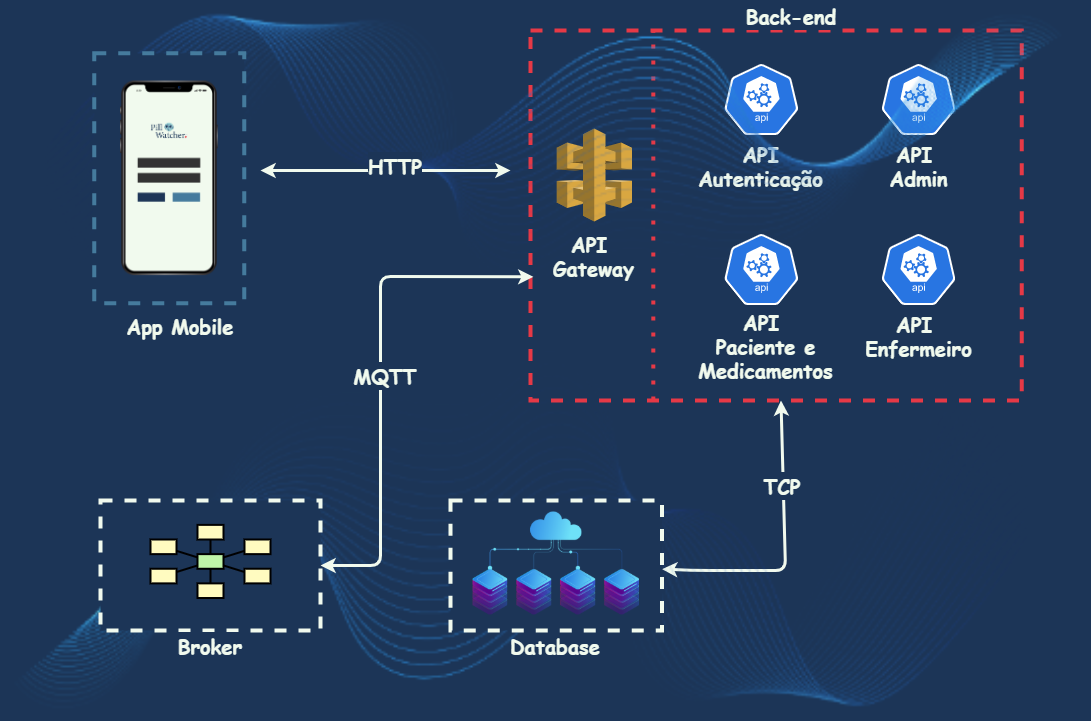
\includegraphics[width=1.0\textwidth]{figuras/solucao_software.png}
    \caption{Solução de Software}
    \label{fig:software_solution}
\end{figure}

\subsection{Banco de Dados}
Para armazenar dados referente à biometria, cadastro de pacientes, medicações, receitas e quaisquer tipo de conteúdos que se relacionam com a solução, optou-se pela utilização da tecnologia de banco de dados MySQL. 

O banco de dados relacional MySQL é um conjunto de dados relacionais, estruturados ou organizados na forma de tabelas, colunas e linhas, onde as tabelas representam os objetos, as colunas representam os campos e as linhas representam os registros \cite{EDUCBA_2020}.

Os dados referentes ao cadastro de medicações, pacientes, enfermeiros, entre outros, serão armazenados na nuvem, utilizando os servidores linux da One Click Hosting. Por outro lado, dados referentes à biometria serão armazenados localmente, dentro da aplicação física, gerenciados pela \emph{Sistema Embarcado}.

O armazenamento na nuvem é adquirido de um fornecedor externo, que tem e opera capacidade de armazenamento físico de dados e entrega essa pela Internet com um modelo de pagamento conforme o uso. Esses fornecedores de armazenamento na nuvem gerenciam a capacidade, a segurança e a resiliência para disponibilizar dados aos aplicativos em todo o mundo \cite{AMAZONWEBSERVICES_2020}.

\subsection{Back-end}
O \emph{Back-end} é a camada onde ocorre o processamento da lógica negocial. É o componente do software que estabelece conexão com a base de dados para registrar e/ou prover informações a um cliente. Tanto a aplicação móvel, quanto ao sistema embarcado instalado no dispensador de remédios se comunicarão com essa camada.

Será desenvolvido com a arquitetura de microsserviços, utilizando o \emph{framework} Spring (Boot, Data, Security) e \emph{libs} (bibliotecas) em Python para a validação de impressões digitais. 
%e aplicação de aprendizado de máquina.
Tais aplicações estabelecerão comunicação entre si através de um sistema gerenciador (API Gateway), utilizando Spring Cloud.

Também será responsável por fazer a integração com o dispensador de medicamentos, utilizando os conceitos de \emph{Internet of Things}. Para essa integração, será utlizado o \emph{middleware} de filas Mosquitto para o repasse e recebimento de informações. As requisições à fila utilizam o protocolo MQTT.

A configuração de ambiente será realizada através da tecnologia Docker. Em ambientes de produção, as aplicações serão implantadas nos servidores em nuvem da One Click Hosting.

\subsection{Front-end}
A aplicação móvel, desenvolvida utilizando o \emph{framework} React Native, proverá uma interface para o gerenciamento dos diversos tipos de usuários. Será responsável também por facilitar o gerenciamento de receitas médicas de seus pacientes e seus respectivos medicamentos, bem como notificar o enfermeiro(a) quando estiver no horário da medicação e quando o estoque de algum medicamento estiver baixo. A aplicação móvel tem como objetivo facilitar a análise de dados através da geração de gráficos e relatórios necessários aos seus usuários. 

Será responsável por validar medicamentos dispensados pela máquina e após esse procedimento, será exibida uma tela onde o profissional confirmará se a medicação foi ministrada ou não.
%Será responsável também por ler um \emph{QR Code} no recipiente que contém o medicamento, para validar que o enfermeiro(a) está entregando a medicação para o paciente correto, no horário adequado.

\subsection{Construção e Entrega de Software}
Para realizar a validação de alterações realizadas em código fonte, optou-se utilizar TravisCI, onde são definidas as etapas descritas abaixo:

\begin{itemize}
    \item \emph{Build}: é construído o código-fonte e verificado se o mesmo está de acordo com padrões de Folha de Estilo pré-definidos;
    \item  \emph{Test}: são realizados os testes unitários e verificados se todos se encontram em estado aprovado;
    \item  \emph{SonarQube Analysis}: o código-fonte é analisado e comparado com métricas de Confiabilidade, Segurança, Manutenibilidade, Cobertura de Testes e Duplicação de Código;
    \item  \emph{Deploy}: a solução é implantada em um ambiente de produção e/ou desenvolvimento. 
\end{itemize}

\begin{figure}[H]
    \centering
    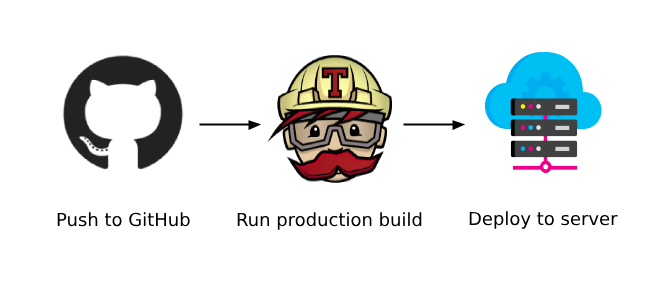
\includegraphics[width=1.0\textwidth]{figuras/deploy-continuous.png}
    \caption{Software Deploy}
    \label{fig:software_deploy}
\end{figure}

A etapa de \emph{Deploy}, listada acima, depende que haja um ambiente pré configurado para ser realizada. Para isso, optou-se utilizar Docker para conteinerização de softwares auxiliares e a One Click Hosting para hospedagem dos serviços em nuvem.

%TODO - Explicar como o software encaminhará as coordenadas da medicação

%Os módulos citados acima serão especificados abaixo, conforme o fluxo de utilização da solução, para que seja possível compreender a importância de cada entregável de software. A cadeia de atividades se dará da seguinte forma:
%\begin{enumerate}
%    \item O usuário com perfil administrador irá cadastrar um enfermeiro na aplicação %\emph{mobile}.
%    \item O enfermeiro cadastrado será responsável por realizar os demais dados cadastrais %na aplicação mobile, como: 
%    \begin{itemize}
%        \item Cadastrar Paciente
%        \item Cadastrar Receita
%        \item Cadastrar Medicação
%    \end{itemize}
%    Durante todo o processo, a aplicação mobile estará conversando com o API Gateway
%    \item O serviço gerenciador (API Gateway) será responsável por encaminhar a informação para o dispensador com as coordenadas da medicação que devem ser liberadas; e, por meio da aplicação mobile, o enfermeiro será notificado entre períodos fixos que existe uma medicação disponível para ser entregue.
%\end{enumerate}

%    \item Matriz de correlação para verificar quais fatores mais interferem na temperatura da %máquina. Os intervalos que estão entre -1 e -0.8; 0.8 e 1 serão mantidos como \emph{features} no %modelo, pois são bons preditores. Uma breve explicação está disponível no Apêndice \ref{MP_app}

\section{Arquitetura de Integração}

\begin{figure}[H]
    \centering
    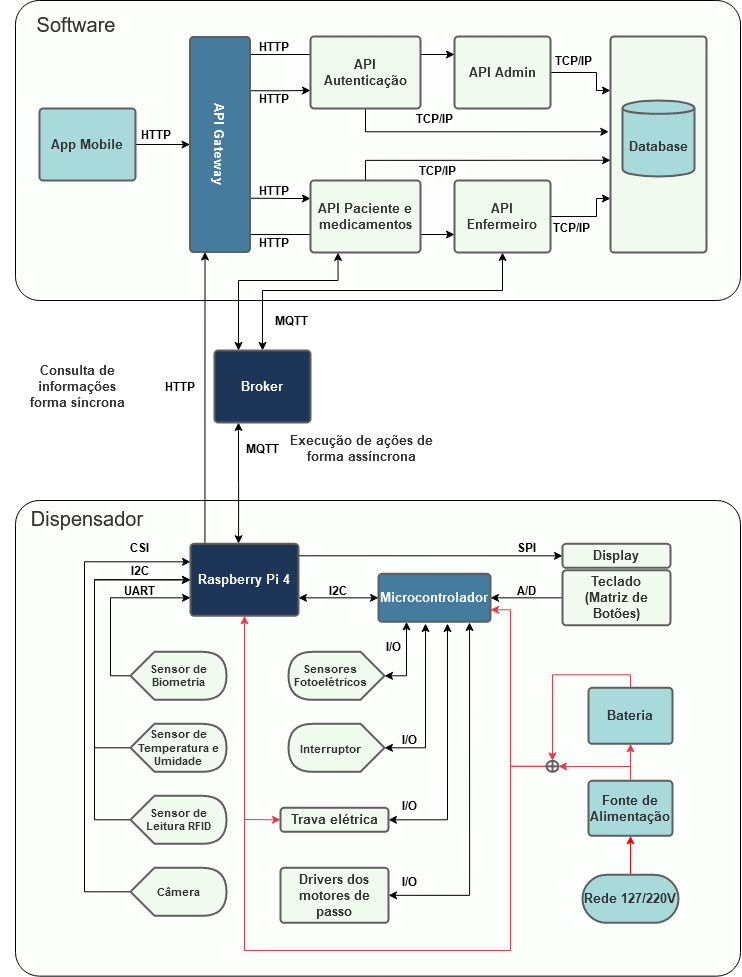
\includegraphics[width=0.9\textwidth]{figuras/diagrama_integracao_v2.png}
    \caption{Arquitetura Inicial entre Eletrônica, Energia e Software}
    \label{fig:fluxograma_integracao}
\end{figure}

